
	In its most basic form, a phase locked loop is a phase-based feedback system whose output tracks or maintains a fixed phase relationship to an input signal. As will be shown, such a system is uniquely suited to the task of frequency synthesis, which is the process of generating derivative frequencies from some reference frequency. Given reference and output phase signals $\Phi_{ref}$ and $\Phi_{out}$, a PLL can be modeled as in figure \ref{fig:basic_fb}, with feedforward and feedback networks A(s) and B(s). 
	\begin{figure}[htb!]
		\center\fontfamily{\sfdefault}\selectfont
% XCircuit output "basic_feedback.tex" for LaTeX input from basic_feedback.ps
\def\putbox#1#2#3#4{\makebox[0.00000in][l]{\makebox[#1][l]{}\raisebox{\baselineskip}[0.00000in][0.00000in]{\raisebox{#2}[0.00000in][0.00000in]{\scalebox{#3}{#4}}}}}
\def\rightbox#1{\makebox[0.00000in][r]{#1}}
\def\centbox#1{\makebox[0.00000in]{#1}}
\def\topbox#1{\raisebox{-0.60\baselineskip}[0.00000in][0.00000in]{#1}}
\def\midbox#1{\raisebox{-0.20\baselineskip}[0.00000in][0.00000in]{#1}}
   \scalebox{1}{
   \normalsize
   \parbox{3.61667in}{
   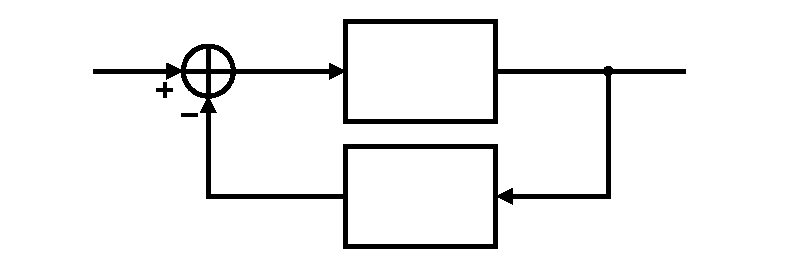
\includegraphics[scale=0.70000]{./figs/basic_feedback.pdf}\\
   % translate x=544 y=496 scale 0.38
   \putbox{1.82000in}{0.85400in}{1.20}{A(s)}%
   \putbox{1.82000in}{0.27300in}{1.20}{B(s)}%
   \putbox{0.44800in}{1.00100in}{1.20}{$\Phi_{ref}$}%
   \putbox{2.84200in}{1.00100in}{1.20}{$\Phi_{out}$}%
   \putbox{1.12000in}{1.00100in}{1.20}{$\Phi_{error}$}%
   } % close 'parbox'
   } % close 'scalebox'
   \vspace{-\baselineskip} % this is not necessary, but looks better
\fontfamily{\rmdefault}\selectfont

		\caption{Basic phase feedback network.}
		\label{fig:basic_fb}
	\end{figure}
	\FloatBarrier
	The closed loop phase response T(s) for $\Phi_{ref}$ to $\Phi_{out}$ is therefore:
	\begin{equation}
		\mathrm{T}(s) = \frac{\Phi_{out}(s)}{\Phi_{ref}(s)} = \frac{A(s)}{1+A(s)B(s)}
	\end{equation}
	A particular case of interest is when B(s) = 1/N, where N is a constant, and the loop gain L(s) = A(s)B(s) $>>$ 1. The closed loop response for this case is:
	\begin{equation}\label{mult_by_n}
		\frac{\Phi_{out}(s)}{\Phi_{ref}(s)} \approx \frac{A(s)}{A(s)B(s)} = \frac{1}{B(s)} = N
	\end{equation}
	We see that the phase through the PLL is multiplied by a factor of N. If the input phase signal is a sinusoid with frequency $\omega_{ref}$, and likewise the output with $\omega_{out}$, then $\phi_{ref}(t)=\omega_{ref}t$ and $\phi_{out}(t)=\omega_{out}t$. Thus:
	\begin{equation}
		\frac{\Phi_{out}(t)}{\Phi_{ref}(t)} = \frac{\omega_{out}t}{\omega_{ref}t} \approx N \hspace{1em} \rightarrow \hspace{1em} \omega_{out} \approx N\omega_{ref}
	\end{equation}
	Therefore, it is observed that a PLL allows for the generation, i.e. synthesis, of a new frequency from a reference frequency signal. Given a feedback divider ratio of 1/N, the PLL multiplies the reference frequency by a factor of N. In the following sections, more advanced models for PLL will be developed, extending the concept introduced here. Specifically, the theory of digital, discrete-time PLLs will be developed and extended from a continuous phase model of a basic PLL.

	\subsection{Continuous PLL Model}
		Although this work is interested in discrete time sampling PLL design, as will later be seen continuous models can still be of use in the analysis and design of such systems. Thus a continuous PLL model is developed in this section.

		\subsubsection{PLL Synthesizer architecture}
			The traditional architecture for implementing a PLL frequency synthesizer \cite{Razavi1996DesignOM} is shown in figure \ref{fig:basic_pll}. This basic PLL is comprised of four components: (1) a phase detector, denoted by PD, (2) a loop filter, denoted by H$_{LF}$(s), (3) a voltage controlled oscillator, denoted by VCO, and (4) and phase divider, denoted by "$\div$ N" in the figure. These components are explained in the following sections.
			\begin{figure}[htb!]
				\center\fontfamily{\sfdefault}\selectfont
% XCircuit output "basic_pll.tex" for LaTeX input from basic_pll.ps
\def\putbox#1#2#3#4{\makebox[0.00000in][l]{\makebox[#1][l]{}\raisebox{\baselineskip}[0.00000in][0.00000in]{\raisebox{#2}[0.00000in][0.00000in]{\scalebox{#3}{#4}}}}}
\def\rightbox#1{\makebox[0.00000in][r]{#1}}
\def\centbox#1{\makebox[0.00000in]{#1}}
\def\topbox#1{\raisebox{-0.60\baselineskip}[0.00000in][0.00000in]{#1}}
\def\midbox#1{\raisebox{-0.20\baselineskip}[0.00000in][0.00000in]{#1}}
   \scalebox{1}{
   \normalsize
   \parbox{4.49167in}{
   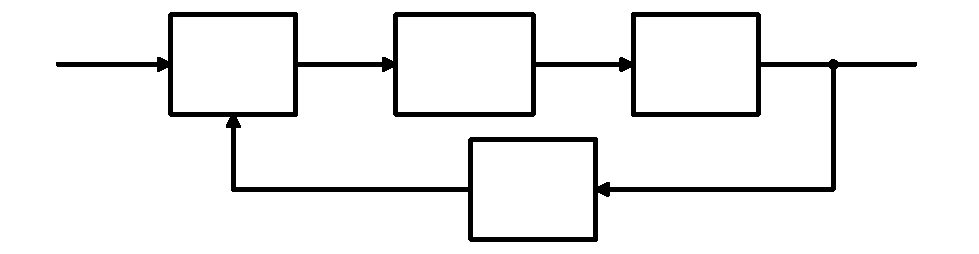
\includegraphics[scale=0.70000]{./figs/basic_pll.pdf}\\
   % translate x=320 y=488 scale 0.38
   \putbox{0.97300in}{0.82600in}{1.20}{PD}%
   \putbox{2.34500in}{0.24500in}{1.20}{$\div$ N}%
   \putbox{0.32900in}{0.97300in}{1.20}{$\Phi_{ref}$}%
   \putbox{3.71700in}{0.97300in}{1.20}{$\Phi_{out}$}%
   \putbox{1.90400in}{0.82600in}{1.20}{H$_{LF}$(s)}%
   \putbox{3.07300in}{0.82600in}{1.20}{VCO}%
   \putbox{1.49800in}{0.39200in}{1.20}{$\Phi_{div}$}%
   \putbox{1.52600in}{0.97300in}{1.20}{$\Phi_e$}%
   \putbox{2.54800in}{0.97300in}{1.20}{V$_{ctrl}$}%
   } % close 'parbox'
   } % close 'scalebox'
   \vspace{-\baselineskip} % this is not necessary, but looks better
\fontfamily{\rmdefault}\selectfont

				\caption{Basic PLL.}
				\label{fig:basic_pll}
			\end{figure}
			\FloatBarrier

		\subsubsection{Divider}
			The phase divider is used as the feedback path in the PLL, where the division ratio N controls the phase and consequent frequency multiplication of the PLL. The transfer function of the divider is:
			\begin{equation}
				\mathrm{H}_{div}(s) = \frac{\Phi_{div}(s)}{\Phi_{out}(s)} = \frac{1}{\mathrm{N}}
			\end{equation}

			\subsubsection{Phase detector}
			The phase detector is used to measure the phase of the feedback signal (i.e. divider output) in relation to the reference phase, in order to establish a phase error signal $\Phi_e$ used to control the tuning of the PLL.
			\begin{equation}
				\Phi_e(s) = \Phi_{ref}(s) - \Phi_{div}(s)
			\end{equation}

		\subsubsection{Loop Filter}
			The PLL loop filter is used to control the phase-frequency response of PLL, which affects transient PLL behavior, as well as phase noise performance (see section \ref{pn_theory}). This can be designed to have P poles and Z zeros, and can be represented in the canonical form of equation \ref{eq:lf_general_form} as a rational function of polynomials of s with coefficients given with $\{a_0, ..., a_P\}$ and $\{b_0, ..., b_Z\}$.
			\begin{equation} \label{eq:lf_general_form}
				\textnormal{H}_{LF}(s) = \frac{\sum_{j=0}^Z b_js^j}{\sum_{k=0}^P a_ks^k}
			\end{equation}
			
		\subsubsection{VCO}
			The voltage controlled oscillator is an oscillator with frequency controlled by an input signal V$_{ctrl}$. The VCO is characterized by its gain $K_{DCO} = \partial f/\partial \textnormal{V}_{ctrl}$, and the nominal oscillation frequency $f_0$. Analyzed in terms of phase, an oscillator can be seen as a time-phase integrator:
			\begin{equation}
				\Phi_{VCO}(t) = \Phi_{out}(t) = \int2\pi(K_{DCO}\textnormal{V}_{ctrl}(t) + f_0)\mathrm{dt}
			\end{equation}
			In the s-domain, where frequency offsets will be represented via initial conditions for modeling purposes, the VCO transfer function is therefore:
			\begin{equation}
				\mathrm{H}_{VCO}(s) = \frac{\Phi_{VCO}(s)}{\textnormal{V}_{ctrl}(s)} = \frac{\Phi_{out}(s)}{\textnormal{V}_{ctrl}(s)} = \frac{2\pi K_{DCO}}{s}
			\end{equation}

		\subsubsection{Continuous PLL Transfer function}\label{cont_pll_tf}
			Now that the continuous PLL synthesizer is understood at a component level, the closed loop dynamics of the PLL can be analyzed. First the PLL loop gain is determined:
			\begin{equation}
				\mathrm{L}(s) = \textnormal{H}_{LF}(s)\textnormal{H}_{VCO}(s)\textnormal{H}_{div}(s) = \frac{2\pi K_{VCO}}{\mathrm{N}}\frac{1}{s}\frac{\sum_{j=0}^Z b_js^j}{\sum_{k=0}^P a_ks^k}
			\end{equation}
			With the phase detector as the feedback summation point, the closed loop response of the PLL from reference to output is in equation \ref{eq:cont_pll_tf}.
			\begin{align} \label{eq:cont_pll_tf}
				\mathrm{T}(s) = \frac{\Phi_{out}(s)}{\Phi_{ref}(s)} = \frac{2\pi K_{VCO}\sum_{j=0}^Z b_js^j}{\sum_{k=0}^P a_ks^{k+1} + \frac{2\pi K_{VCO}}{\mathrm{N}}\sum_{j=0}^Z b_js^j} = \mathrm{N}\frac{\mathrm{L}(s)}{1 + \mathrm{L}(s)}
			\end{align}

